\documentclass{llncs}
%
\usepackage{makeidx}  % allows for indexgeneration
\usepackage{booktabs}
\usepackage[colorinlistoftodos]{todonotes}
%\usepackage{graphicx}
%\usepackage{caption}
%\usepackage{subcaption}
%
\begin{document}
%
\frontmatter          % for the preliminaries
%
\pagestyle{headings}  % switches on printing of running heads
\addtocmark{Active Global Address Space} % additional mark in the TOC
%
%
\mainmatter              % start of the contributions
%
\title{Assessing the Performance Impact of an Active Global Address Space}
%
\titlerunning{Hamiltonian Mechanics}  % abbreviated title (for running head)
%                                     also used for the TOC unless
%                                     \toctitle is used
%
\author{Parsa Amini\inst{1}, Hartmut Kaiser\inst{2}, \and Jeanine Cook\inst{3}}
%
\authorrunning{Parsa Amini et al.} % abbreviated author list (for running head)
%
%%%% list of authors for the TOC (use if author list has to be modified)
\tocauthor{Parsa Amini, Hartmut Kaiser, Jeanine Cook}
\institute{
\email{parsa@cct.lsu.edu},
\and
\email{hkaiser@cct.lsu.edu}
\and
\email{jeacook@sandia.gov}}

\maketitle              % typeset the title of the contribution

\begin{abstract}
%\todo[inline, color=red!50]{What is this?}%
%\todo[inline, color=red!50]{What do we talk about?}%
In this research, we describe the functionality of AGAS, a subsystem of the HPX
runtime system that is designed to handle data, independent of the hardware and
architecture configuration. AGAS enables runtime global data access and data
migration, but incurs a an overhead cost at runtime. We present
a method to assess the performance of AGAS and the amount of impact
it has on execution of the OctoTiger application. With our assessment method we identify
three problematic spots in the HPX version used in our experiments.


%data during
%runtime means a portion of the application execution time is spent executing
%AGAS code. To assess AGAS's performance we introduce and present a method using
%data that can be gathered using HPX's Performance Counter framework. We apply
%this method on a strong scaling experiment running an AMR application called
%OctoTiger and present our measurements.
\end{abstract}

%\keywords{HPX, AGAS, PGAS}
\begin{IEEEkeywords}
HPX, AGAS, PGAS
\end{IEEEkeywords}


%
\section{Introduction}
Global address space systems attempt to boost productivity and simplify the
application development cycle of distributed applications by providing a
ubiquitous abstraction layer over memory spaces that are provided and managed
by the operating system on each node in a large-scale system. SPMD-style (Single Program Multiple
Data) Partitioned Global Address Space designs eliminate this layer during
compilation to avoid the complexity of resolving global addresses at runtime at
the cost of limiting productivity and imposing limitations on the code, while
others like HPX\cite{Kaiser2014,hpx_repo}, HPX5\cite{hpx5},
Charm++\cite{Kale1993}, UPC++\cite{Zheng2014}, and Chapel\cite{chapel_lang} provide a
runtime component that maps global addresses to virtual addresses during
application execution to provide true global addresses.


The demand for models that enable applications to process massive
datasets within specific time, power, and budgetary constraints continues to
pose challenges for the computer science community
\cite{Amarasinghe091exascale,Sterling2009}. One category of such complexities
includes managing a large quantity of objects across several machines and
memory partitions while maximizing data locality. Several Partitioned Global
Address Space systems (PGAS) \cite{pgasorg} try to address these needs by
providing control over data distribution and facilitating data accesses across
processes and machines. However, initial data placement alone is not sufficient
%\todo{What does AGAS enable? Reduced data movement. Reduced latency because an access to a non-local object is faster than accessing memory? Why should the reader care about AGAS?}
%\todo{AGAS should be more strongly motivated. How do you know that scaling impared applications are impared by poor data locality}
to address more complex issues such as load balancing applications that run on heterogeneous clusters or applications
that become scaling impaired over time due to increasing load imbalance like
adaptive mesh refinement (AMR), dynamic graph applications, and partial
differential equation (PDE) solvers\cite{5364511,Anderson2011a,Dekate2011}.
Active Global Address Space (AGAS) is a system that tries to address
performance impaired applications. AGAS was initially proposed for the ParalleX
programming model\cite{5364511} and implemented in HPX. It adds an abstraction
layer on top of local objects on each compute node by mapping local virtual
addresses to a global address and ensuring that global addresses are valid even
if the object it refers to is migrated to a different physical location. AGAS
enables applications to perform load balancing at runtime by using data
migration.  AGAS also reduces data movement by using active messages. Active
messages significantly reduce the need for data movement by moving tasks to
where the data is instead of moving the data to where work is. 
%This enables AGAS to provide data migration for load balancing performance impaired applications.
However, AGAS needs to execute code to resolve and maintain the references and
takes a portion of the execution time.
%\todo{Talk about reducing the impact of AGAS overhead}


Assessing the overheads caused by AGAS is the main objective of this paper. We
address this objective by developing a system that uses measurement data from
AGAS and apply it to identify AGAS functions that exhibit poor scaling
behavior in HPX 0.99. In the rest of this work, we discuss other pertinent
research in section \ref{related_work}, present a general overview of AGAS
functionality in section \ref{agas}, explain the criteria based on which the
results can be evaluated in section \ref{performance}, experiments that were
run and examine their results in section \ref{results}, and further analyze
them and consider directions that are likely to produce more insights into
improving AGAS considering our findings in section \ref{conclusions}.

\section{Related Work}
\label{related_work}

%\todo{You need a section on background of global address spaces, why they are needed, how do they work? Not everyone knows this.}
The MPI programming model provides the user with complete control over data
locality and performance. On the other hand, it does not have the
programmability and data referencing simplicity of shared-memory systems. The
global address space model combines the two models and enables processes to
access shared memory locations with a global address while maintaining an
explicit distinction between local and remote operations. This provides the
means to implement distributed versions of commonly used data structures like
arrays, sets, matrices, or any data structure that is based on pointers.

Some global address space implementations like Unified Parallel C (UPC)\cite{upc_org}, Co-Array
Fortran, Titanium\cite{yelick1998titanium}, and SHMEM\cite{shmem_feind1995,openshmem_chapman2010}, the global addresses are resolved to communication calls
during compilation. Because global address resolution is performed at compile
time, these implementations still do not provide the freedom programmers have
in a shared memory application. Additionally, they still use global barriers as
the synchronization mechanism, which does not trivially achieve shared memory
applications performance.

Asynchronous PGAS implementations (e.g. Charm++, UPC++, Chapel, and X10) follow
the asynchronous many task model to dynamically perform load balancing at
runtime. They allow multiple tasks to run within each operating system thread
and provide tools for controlling the memory layout and expressing
multidimensional, sparse, associative, or unstructured data structures.

In recent years, there has been a significant increase in utilization of
heterogeneous clusters that use GPUs and MICs in addition to
CPUs\cite{Lena2014,Yang2011266,Potluri2014,Sidelnik2011}. One approach to
manage such systems is using
solutions\cite{Rabenseifner2009,Yang2011266,Chorley2010} that separately use a
library like MPI for explicit communication between nodes and a choice of
shared-memory programming framework such as OpenMP\cite{openmp_org}, Kokkos\cite{kokkos_paper,kokkos_repo}, or
UPC. Other approaches include Asynchronous PGAS
runtimes\cite{Saraswat2010} and Charm++ that use dynamic
multithreading to avoid fragmenting the application development process to
separately manage communication and computation while maintaining portability
between various cluster configurations and providing access to heterogeneous
computing resources\cite{P0234R0}.

Most studies on distributed runtime systems do not include quantitative
analysis of the performance of their global address space system but present
the overall performance of applications using the respective model or
implementation. However, amongst the runtime systems mentioned only HPX has a
global address system that allows objects to be relocated at runtime. This
unique property calls for a closer look into HPX's Active Global Address Space
system behavior and performance and is the motivation behind this study.

\section{Active Global Address Space}
\label{agas}

This section provides an overview of the implementation of the Active Global
Address Space (AGAS) in HPX runtime system.

AGAS is a global memory addressing system that is designed to
handle various memory configurations ranging from those implemented in single small
machines to those typically found in a cluster composed of a large number of
nodes with heterogeneous computing resources. AGAS is designed such that
specific memory configuration characteristics are handled by the programmer
through the API. Fig.
\ref{fig:agas_struct} illustrates AGAS's role in HPX. Typically, 
each part of the distributed AGAS service is hosted on a separate node of a
cluster.

AGAS consists of several subsystems that are depicted in Fig.
\ref{fig:agas_intern} and are the following:

\begin{figure*}[t]
    \centering
    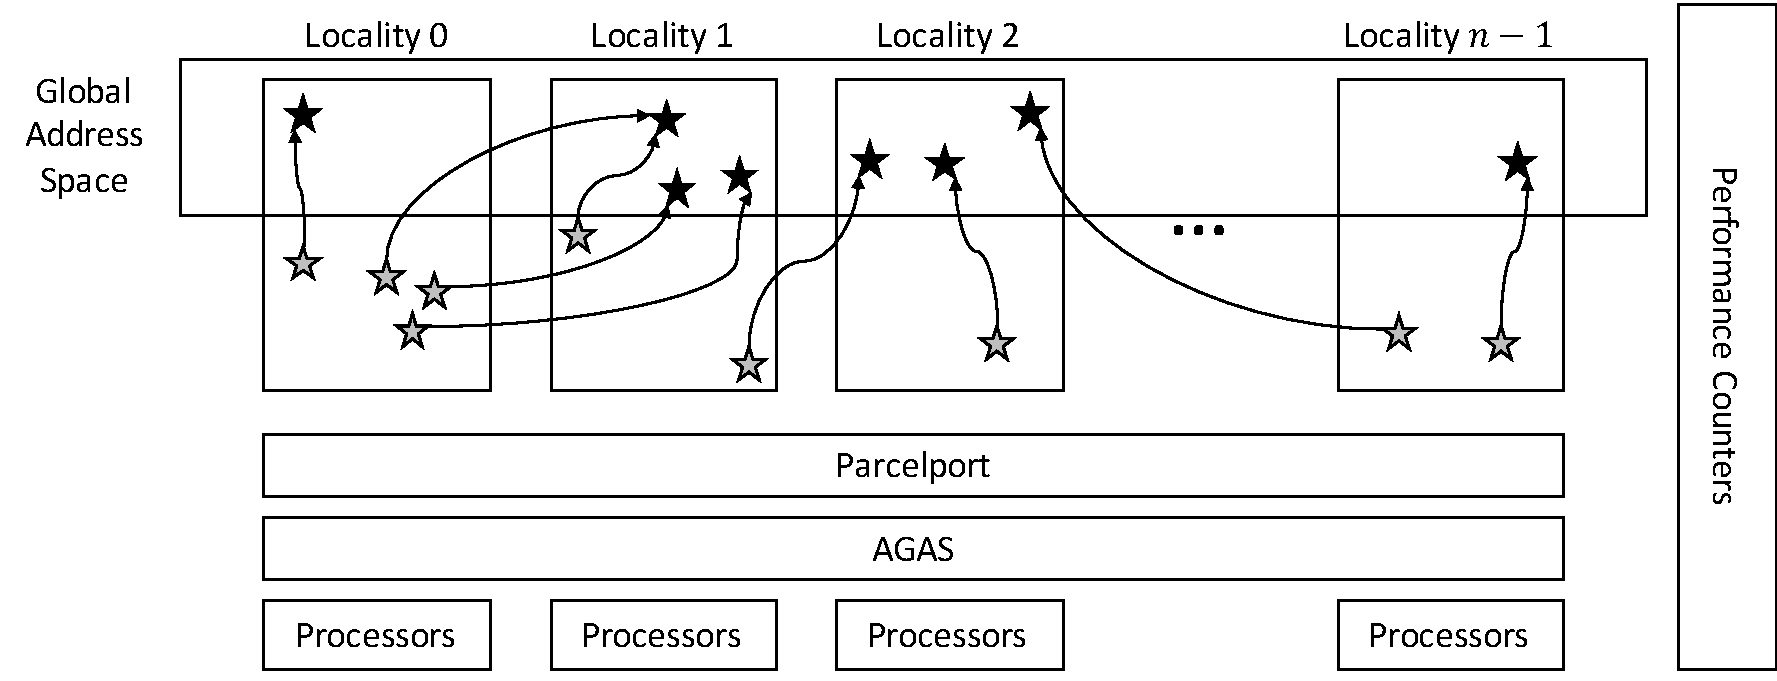
\includegraphics[width=.9\textwidth,height=\textheight,keepaspectratio]{illustrations/agas_struct}
    \caption{AGAS provides an abstraction layer on top of virtual addresses local to each locality. Global objects are shown as black stars and gray stars indicate references to global objects. Each reference is connected to global objects by an arrow.}
    \label{fig:agas_struct}
\end{figure*}
\begin{figure*}[t]
    \centering
    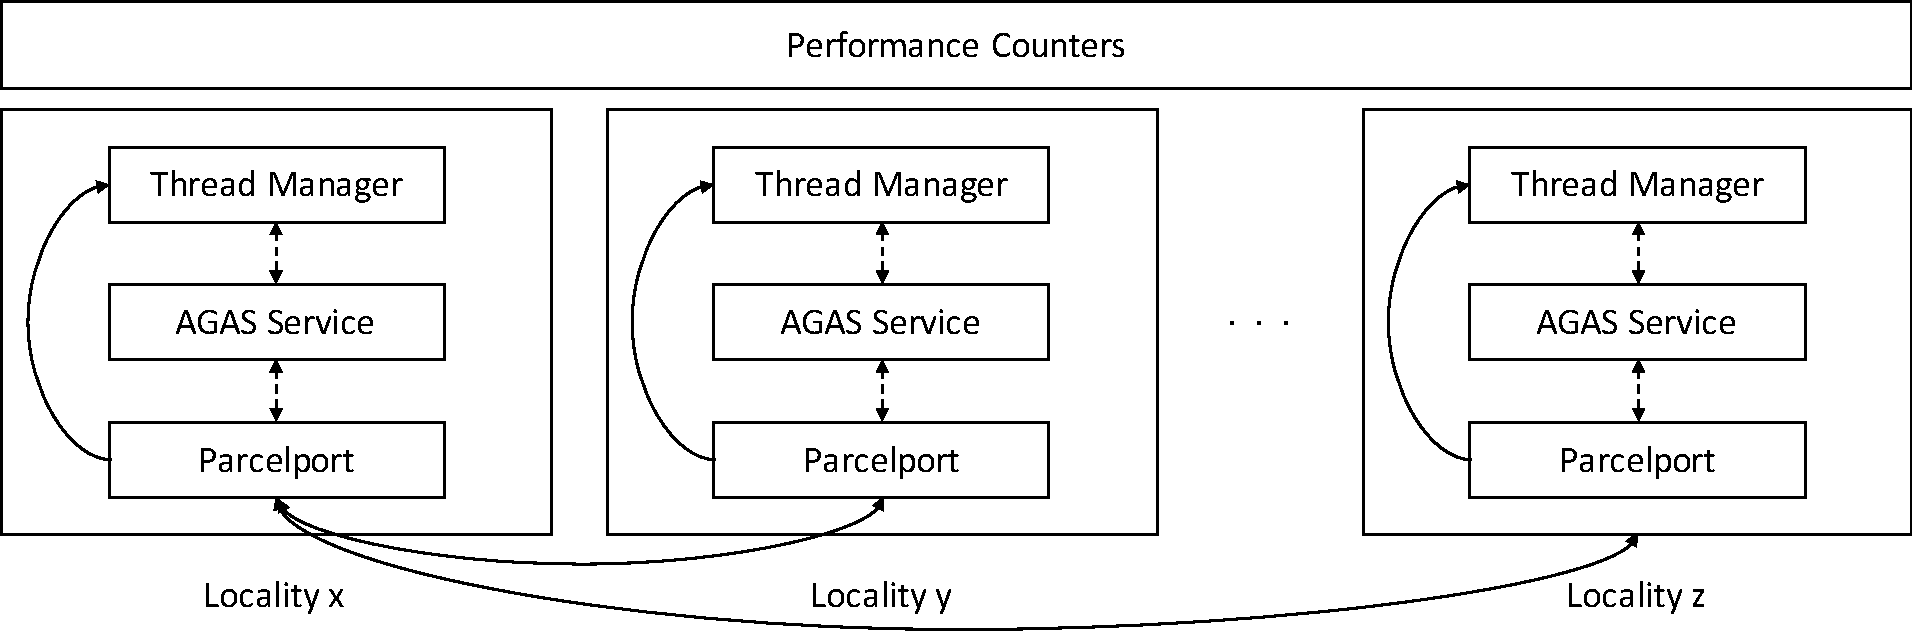
\includegraphics[width=.9\textwidth,height=\textheight,keepaspectratio]{illustrations/agas_interaction}
    \caption{When an HPX thread accesses a global object, AGAS determines if the object can be accessed locally. If the object is on a different locality the HPX thread is serialized and given to the parcelport. The parcelport unserializes the task and hands it to the thread manager for execution.}
    \label{fig:agas_interaction}
\end{figure*}

%\begin{figure*}[t!]
%    \centering
%    \begin{subfigure}[t]{.5/\textwidth}
%        \centering
%        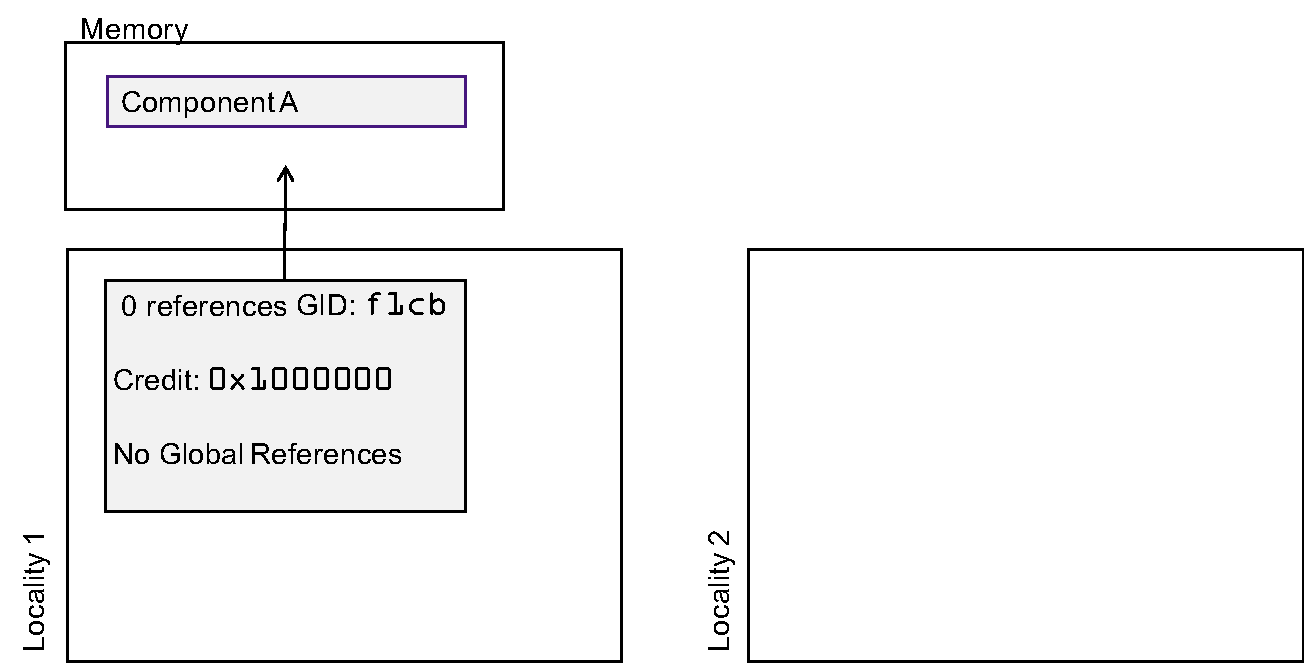
\includegraphics[width=.49\textwidth,height=\textheight,keepaspectratio]{illustrations/reference_counting_1}
%        \caption{}
%    \end{subfigure}
%    \label{fig:agas_ref_count_1}
%\end{figure*}

\begin{enumerate}
    \item{Primary Namespace:
        To provide uniform access to objects across the boundaries
        of physical partitions in a cluster, AGAS provides applications
        with 128-bit global identifiers (GIDs) to be used in place of
        virtual addresses that are local to specific nodes.
        Consequently, AGAS maintains mapping tables to be able to map GIDs
        to local virtual addresses.}
    \item{Locality Namespace:
        Information about the nodes and computing resources allocated to
        each physical partition is held in the locality namespace. Each 
        partition is called a "locality" and locality 0 is responsible for 
        maintaining current information about all other localities.}
    \item{Component Namespace:
        Types are registered in this namespace to facilitate resolving resource 
        requirements during bulk memory allocations.}
    \item{Symbolic Namespace:
		The symbolic namespace is a layer on top of the global address space
		that allows mapping symbolic names to global addresses for the purpose
		of resolving global addresses at runtime. This is useful in cases where
		data about specific events needs to be collected. For example, HPX
		performance counter system uses the symbolic namespace for collecting
		performance counter data.}
    \item{AGAS Cache:
		AGAS cache stores mapping between the most recently used global
		addresses to localities where those object reside and local virtual addresses. If a task requires
		an object that does not live on the same locality then the task is sent
		to the locality where the object currently is. However, in order to do
		so, AGAS has to determine the current location of the queried object.
		If AGAS does not know the current location then it forwards the query
		to the locality where the object was originally created. The locality
		on which an object is created stays responsible for maintaining the
		current location of the object during its entire lifetime. If an object
		is likely to be accessed again then the locality that forwards a task
		will also request the original locality to report the object's current
		location. This information is stored in the AGAS cache. The AGAS cache
		is small since it is designed for speed and therefore, it does not know
		all local objects.}
    \item{Garbage Collection:
        A distributed garbage collection system tracks objects during their
        lifetime and frees the consumed memory when an object goes out of
        scope and therefore can no longer be accessed in the program. HPX
        complies to the C++ standard specifications and hence, it provides
        structures similar to what the modern C++ standard requires.
        Additionally, GIDs in HPX can be managed or unmanaged and in case of
        the former AGAS tracks that GID until the reference is lost so that it
        can free up the memory space when possible. AGAS uses reference
        counting to determine if there are existing references to an object and
        a credit-based scheme for remote references. The local counter is
        updated when a new reference is created and when a reference goes out
        of scope on the same locality. As for remote references, the credit
        system works as demonstrated in Fig. \ref{fig:agas_credit}}

        \begin{figure*}[t]
            \centering
            \begin{subfigure}[t]{0.49\textwidth}
                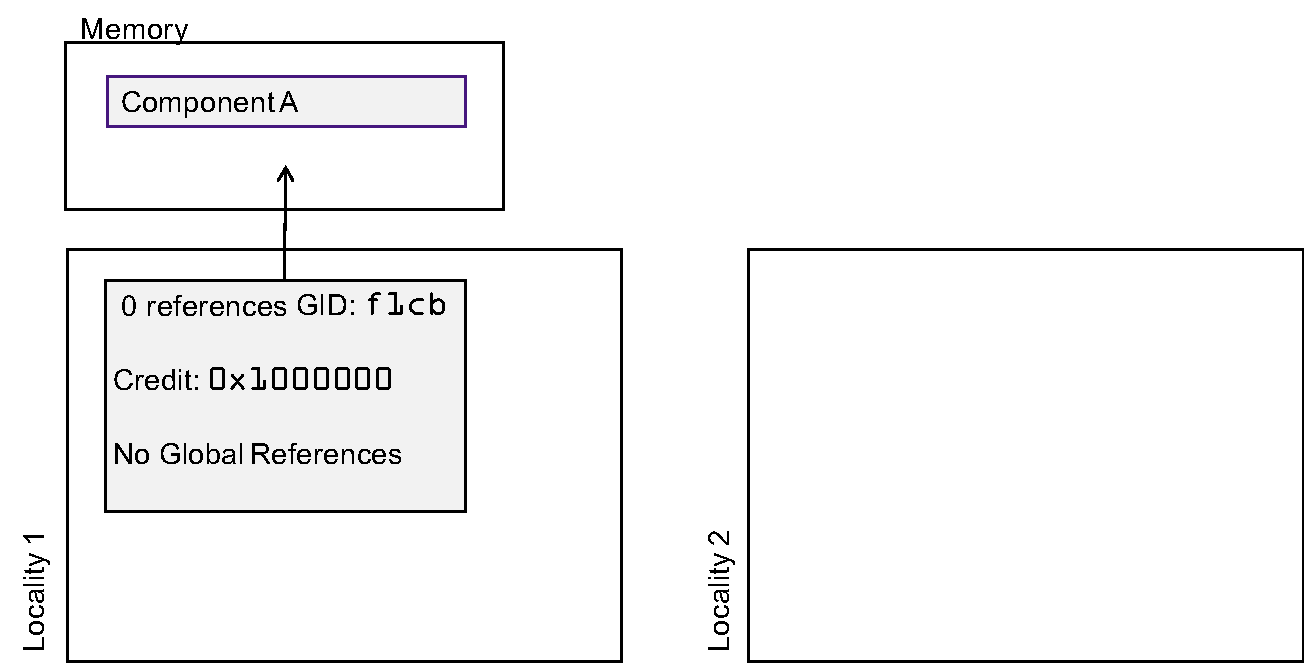
\includegraphics[width=\textwidth]{illustrations/reference_counting_1}
                \caption{An object is created. AGAS sets the object's credit to a large
                  number.}
                \label{fig:agas_credit_1}
            \end{subfigure}
            \vspace{2em}
            \hfill
            \begin{subfigure}[t]{0.49\textwidth}
                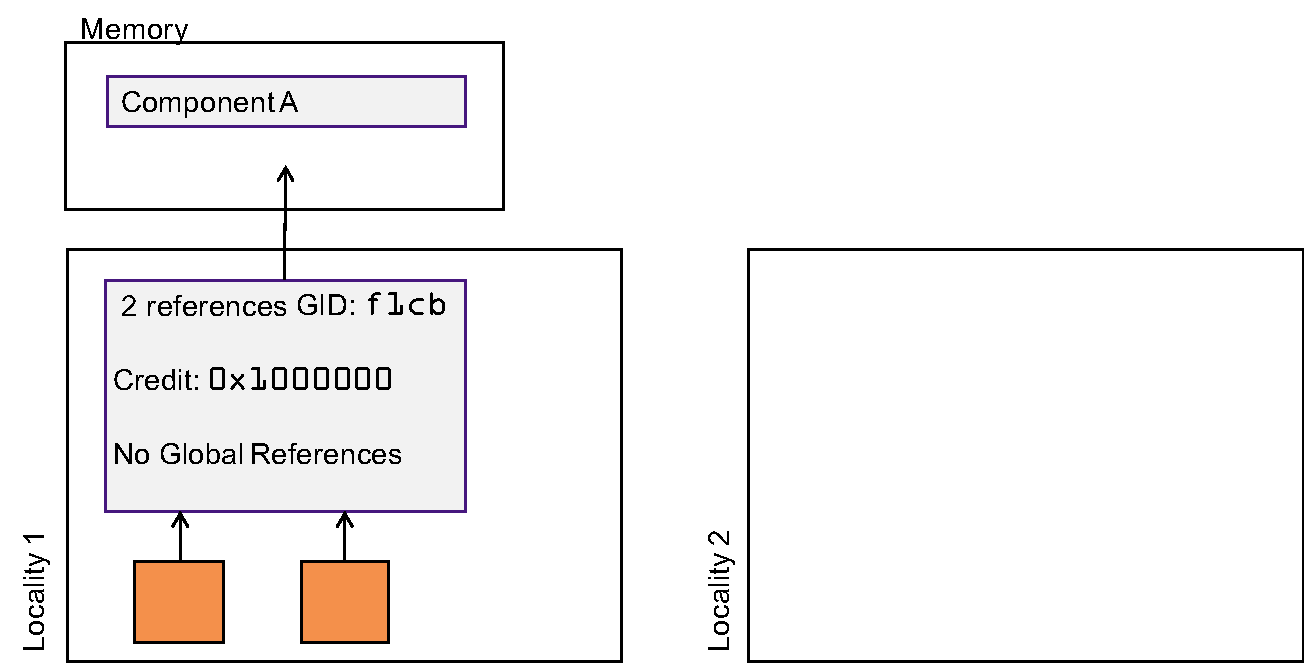
\includegraphics[width=\textwidth]{illustrations/reference_counting_2}
                \caption{A global object referenced by two local copies of the GID. Credit is not affected by local copies.}
                \label{fig:agas_credit_2}
            \end{subfigure}
            \begin{subfigure}[t]{0.49\textwidth}
                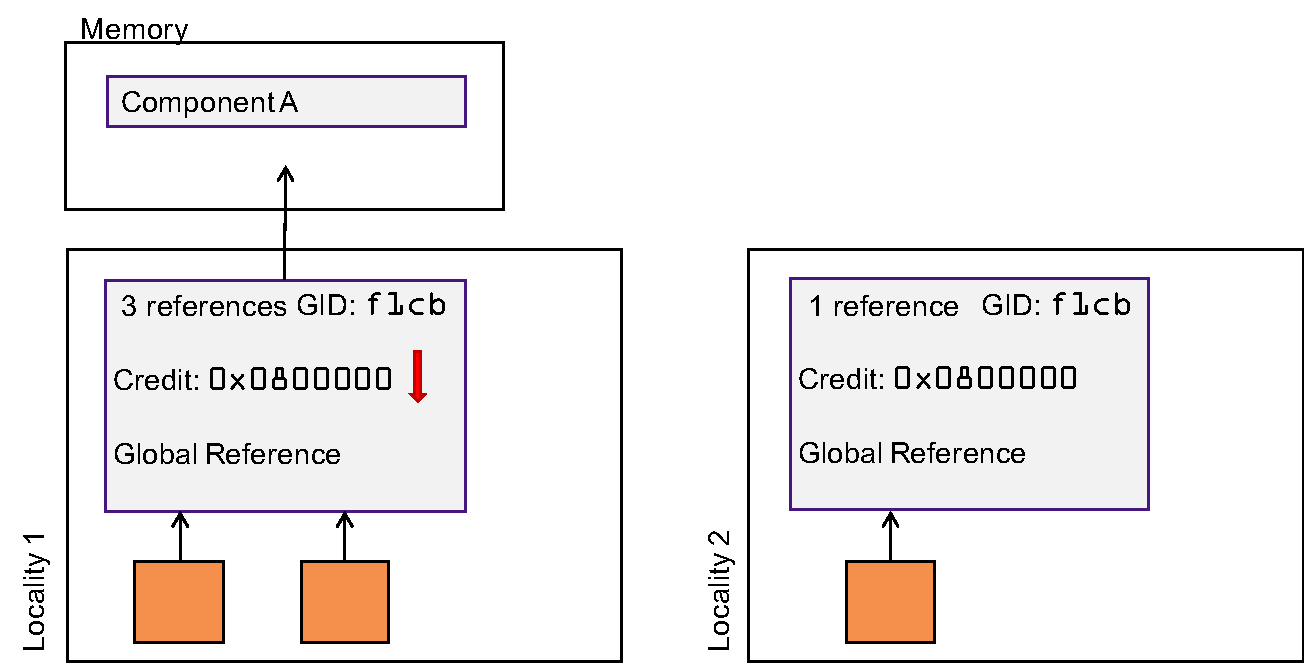
\includegraphics[width=\textwidth]{illustrations/reference_counting_3}
                \caption{When an object is referenced by another locality the object's
                  credit is split in half and a copy of the reference is kept at both
                  localities, and a flag is set on the original reference to
                  indicate that the object is referenced globally. When a copy
                  runs out of credit, it will ask the lender AGAS instance (the
                  locality where the reference is located) for more. If the
                  original reference itself does not have enough credit, the
                  AGAS instance responsible for that reference (where the
                  object resides) will grant it more credit.
                }
                \label{fig:agas_credit_3}
            \end{subfigure}
            \hfill
            \begin{subfigure}[t]{0.49\textwidth}
                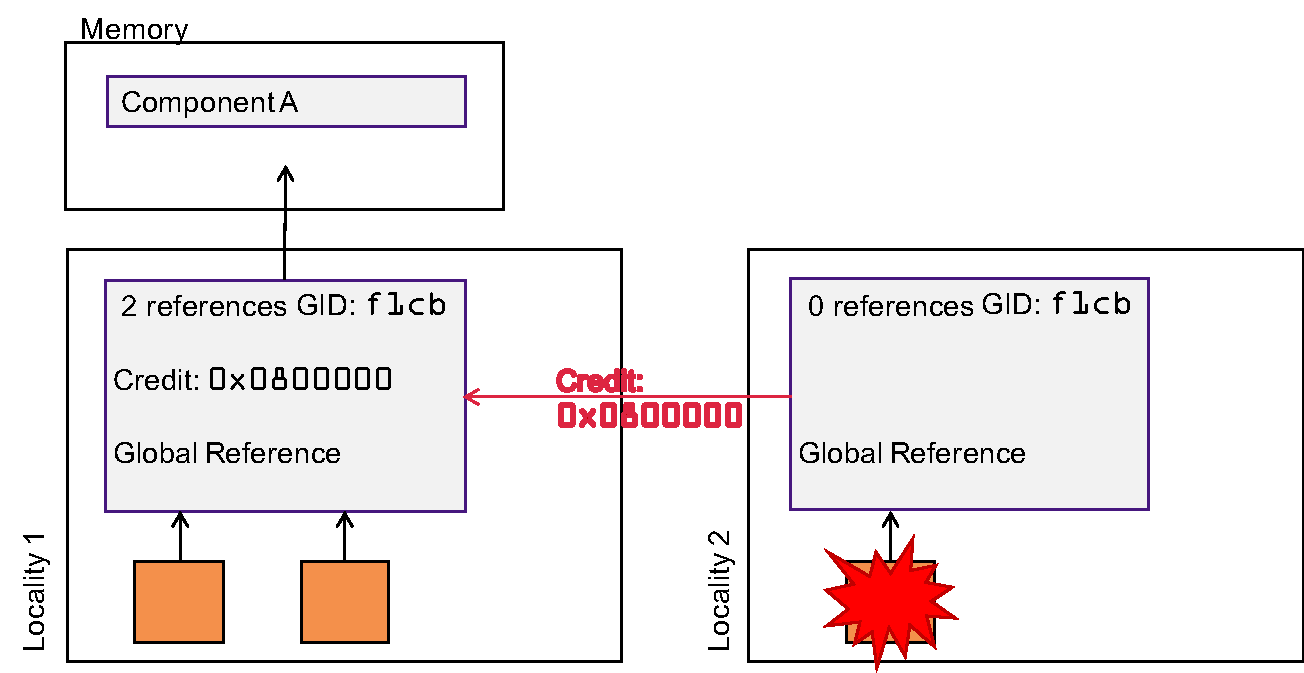
\includegraphics[width=\textwidth]{illustrations/reference_counting_4}
                \caption{When a reference goes out of scope AGAS returns all borrowed
                  credits to the original reference. If there are no local references and all credits have been
                  returned then AGAS can remove the object from memory during garbage
                  collection.}
                \label{fig:agas_credit_4}
            \end{subfigure}
            \caption{AGAS credit system tracks global references. When a global reference goes out of scope all of its credit is returned to the lender. When there are no local or global references the memory allocated by the object can be freed by the garbage collector.}
            \label{fig:agas_credit}
        \end{figure*}
\end{enumerate}

\begin{figure*}[t]
    \centering
    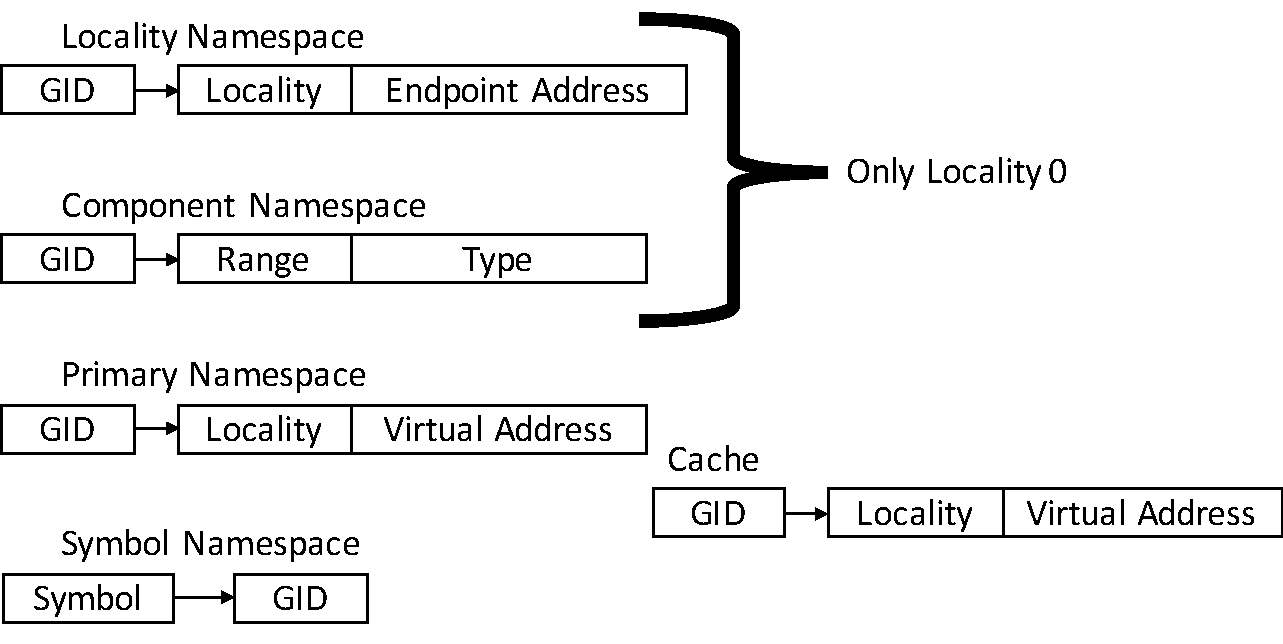
\includegraphics[width=.9\textwidth,height=\textheight,keepaspectratio]{illustrations/agas_intern}
    \caption{The four namespaces inside AGAS. Primary namespace on each AGAS instance contains GID to local address mappings. Locality namespace holds information about all AGAS instances. Component namespace tracks bulk memory allocations dedicated to types. Symbolic namespace contains mappings between GIDs and special strings that can be used for various purposes such as facilitating the collection of data about application execution.}
    \label{fig:agas_intern}
\end{figure*}

Garbage collection at runtime requires execution of code that is otherwise not
present and consumes computing resources. Performing garbage collection
requires executing code that is the not the user's application. AGAS tries to
minimize garbage collection sweeps by performing it when the volume of garbage
reaches a certain threshold that can be specified by the users. It is also
possible to manually initiate it inside applications by developers.

When the code accesses the object referred to by a GID, AGAS looks up the GID
in the primary namespace and returns the local virtual address for the object
if the object lives on the same locality. As for remote objects, AGAS interacts
with the parcelport service to resolve the remote reference access as shown in
Fig. \ref{fig:agas_interaction}. This design hides the communication latencies
by resolving the remote reference accesses asynchronously.

\subsection{AGAS Performance Counters}
HPX is a runtime system that includes novel abstractions on top of ordinary
operating systems and hardware that are more difficult to benchmark using traditional
performance measuring tools such as hardware performance counters included in
Intel processors. HPX introduces a set of performance counters to let
developers monitor the performance of its subsystems, including AGAS, during
execution. This allows the users to use performance counters to debug their
code and locate performance bottlenecks. Users can also develop their own
performance counters to retrieve arbitrary information during execution.

Performance counters can be queried at runtime. For example, APEX\cite{JSFI64}
uses data provided by the performance counter system at runtime to make
decisions in its policy engine to perform autotuning on the running HPX
application and improve execution time. It is also possible to ask HPX to print
the performance counter data.

Similar to hardware performance counters, HPX performance counters\cite{grubel2015performance} are designed
to expose performance data on the underlying function calls. HPX has
performance counters that measure performance of AGAS subsystems. Each AGAS
performance counter either reports the number of invocations or the total
execution time of the selected operation.

\subsection{Migration}
Objects registered in AGAS can be physically moved to a different locality
while retaining the same address. Moreover, this operation does not need the
application execution to be suspended. After a global object is relocated to
the new locality, all reference accesses that try to access the object are
forwarded to the new locality and their localities are notified of the move.

Migration is an especially useful feature for applications that suffer from
poor data locality and/or are balance impaired and it can be used to adaptively
improve data locality when scaling is being hurt.

\subsection{HPX bootstrap and teardown}
Before an HPX application can start executing, HPX has to initialize. This
process is called bootstrap and includes registering runtime services, data
types, performance counters, and symbols.
Similarly during teardown, after applications built with HPX complete, HPX removes all
objects, frees all allocated hardware resources and may perform additional
tasks such as collecting performance counter data when applicable.

In this research, we exclude data from the bootstrap and teardown phases since
they do not directly provide useful data on how AGAS might impact the
performance or scaling behavior during runtime.

\section{Quantifying AGAS Performance}
\label{performance}

The main challenge of any HPC global addressing system, including AGAS, is to
efficiently support the massive amounts of data that applications use during
execution. Our aim here, therefore, is to understand the efficiency of AGAS
through measuring its performance of associated overheads.
To study AGAS, we use OctoTiger\cite{kadam2017numerical,heller2017harnessing,octotiger_repo} as our
application and run it on the cluster provided by the Center of Computation and
Technology at Louisiana State University. It has to be noted that any other
application benchmark can be used in place of OctoTiger. However, developing an
HPX application takes work and at this point, OctoTiger is the only
available real world HPX application. In the rest of this section we present
OctoTiger and the performance metrics we use to measure the overheads
of AGAS. 

\subsection{OctoTiger}
%\todo[inline, color=red!50]{What is it? Why did we choose it? What are the implications of this choice?}%
LSU OctoTiger is a state of the art multi-physics AMR HPX application that
simulates the merger of double white dwarf binaries. Its computations include
hydrodynamics, gravitational, and radiation transportation solvers. It fully
utilizes the capabilities of AGAS in HPX since it dynamically changes the
computational resolution based on the actual needs of the simulation and thus, 
it is an inherently balance impaired application. It is also a memory intensive
application compared to most exascale challenge problems. For example,
Quicksilver and Pennant from CORAL2 benchmarks have a high water mark of 16\%
and 8\%, respectively, whereas for OctoTiger this number is about 60\%.

We use OctoTiger to study the behavior of AGAS when used by applications
running on large machines. We ran our experiments on SuperMIC at Louisiana
State University, a hybrid cluster composed of Xeon, Xeon Phi Knights Corner, 
and NVIDIA Tesla processors. Due to the complexity of the computations
performed by OctoTiger, adjusting the size of the problem with reasonable
accuracy to demonstrate weak scaling is not practical and therefore we
presenting the impacts of strong scaling on AGAS behavior.

\subsection{System and Environment Setup}
%\todo[inline, color=red!50]{Where are the experiments run? Why? What are the implications of this choice?}%
We run our experiments on SuperMIC, a hybrid Xeon/Xeon Phi cluster that
comprises 360 compute nodes located at Louisiana State University. More
details about the configuration of SuperMIC is included in Table
\ref{tab:machines}. We run OctoTiger on SuperMIC from
two nodes to 194 nodes only using the Xeon processors on each machine using
HPX 0.9\cite{hartmut_kaiser_2015_33656}.

% Sample LLNCS table
%\begin{table}
%    \caption{SuperMIC Configuration}
%    \label{tab:machines}
%    \begin{center}
%    \begin{tabular}{r@{\quad}rl}
%    \hline
%    \multicolumn{1}{l}{\rule{0pt}{12pt}
%                       Year}&\multicolumn{2}{l}{World population}\\[2pt]
%    \hline\rule{0pt}{12pt}
%    8000 B.C.  &     5,000,000& \\
%      50 A.D.  &   200,000,000& \\
%    1650 A.D.  &   500,000,000& \\
%    1945 A.D.  & 2,300,000,000& \\
%    1980 A.D.  & 4,400,000,000& \\[2pt]
%    \hline
%    \end{tabular}
%    \end{center}
%\end{table}

\begin{table}
    \caption{SuperMIC Configuration}
    \centering
    \label{tab:machines}
    \begin{tabular}{cl}  
        \toprule
        Nodes available  & 360                             \\
        Architecture     & Ivy Bridge,                     \\
                         & Knights Corner                  \\
        Cores/Node       & $2 \times 10$ cores             \\
        Processor        & Intel Xeon E5-2680 @ 2.8 GHz,   \\
                         & Intel Xeon Phi 7120P @1.238 GHz \\
        Memory           & 64 GB DDR3 @ 1,866 MHz          \\
                         &                                 \\
        Connection       & 56 Gbps Infinitband             \\
        Operating System & Red Hat Enterprise Linux 6.8    \\
        \bottomrule
    \end{tabular}
\end{table}

\begin{itemize}
\item{Performance Metrics}:
Every globally accessible object in HPX has a global ID that AGAS manages and
resolves to local virtual addresses at runtime. However, address resolution at runtime is
an overhead that consumes computational resources that application developers expect to be used by the
applications rather than the runtime system. To quantify and study the overhead of AGAS, we look at the following
fundamental operations, the number of calls, and the amount of time that is
spent performing these operations.

\item{Bind, Unbind, Object Lookup}:
Bind and Unbind operations occur when a global object is created and deleted, 
respectively. An object lookup operation takes place each time AGAS attempts 
to resolve a global ID.

\item{Locality Lookup}:
Each AGAS instance only knows about itself and locality 0. When an AGAS
instance needs to communicate with another locality and does not have
information about the appropriate communication endpoint to do so, it needs to
query that information from locality 0.

\item{Parcel Routing}:
HPX implements active messages in the form of parcels\cite{wagle2018methodology}. A parcel is packaged
information that triggers an operation upon reception by an AGAS instance. For
example, when an HPX task needs to operate on information that resides on
another locality, AGAS serializes the task along with its arguments and state
information and forwards it to the locality on which data resides.

\item{Cache}:
Whenever AGAS decides that an address is likely to be queried again, it stores
that information in the local AGAS cache of that locality. To serve its purpose of actually improving
performance the AGAS cache is designed to hold a limited number of entries that is
defined by user configuration.

\item{Garbage Collection}:
\label{sec:garbage_collection}
HPX provides managed objects whose lifetime is controlled by the garbage
collection mechanism instead of the programmer having to free the memory
consumed by each object. HPX uses reference counting to track references local
to each AGAS instance and a credit scheme to manage global references. Once an
object no longer has any local references and/or all its global reference
credits are returned, it is deemed garbage and is collected when the garbage
collection operation is triggered by reaching a certain threshold or by the
application developer in their code. Registration and removal of global references is done by
calling \textit{increment\_credit} and \textit{decrement\_credit} functions, respectively.
\end{itemize}

\section{Performance Results}
\label{results}

As mentioned before, the main objective of this study is to identify the AGAS
operations that need performance improvement and to study the effects of strong
scaling on AGAS. In this section, we present the results of this study.

\begin{figure}[h]
    \centering
    \caption{Total time spent to resolve GID calls while running OctoTiger on 32 to 200 nodes of SuperMIC with fixed problem size (Strong Scaling). Each (red) circle refers to the measured amount of time a locality has spent executing resolve GID calls. Higher intensities indicate overlapping measurements. The line highlights locality 0's behavior.}
    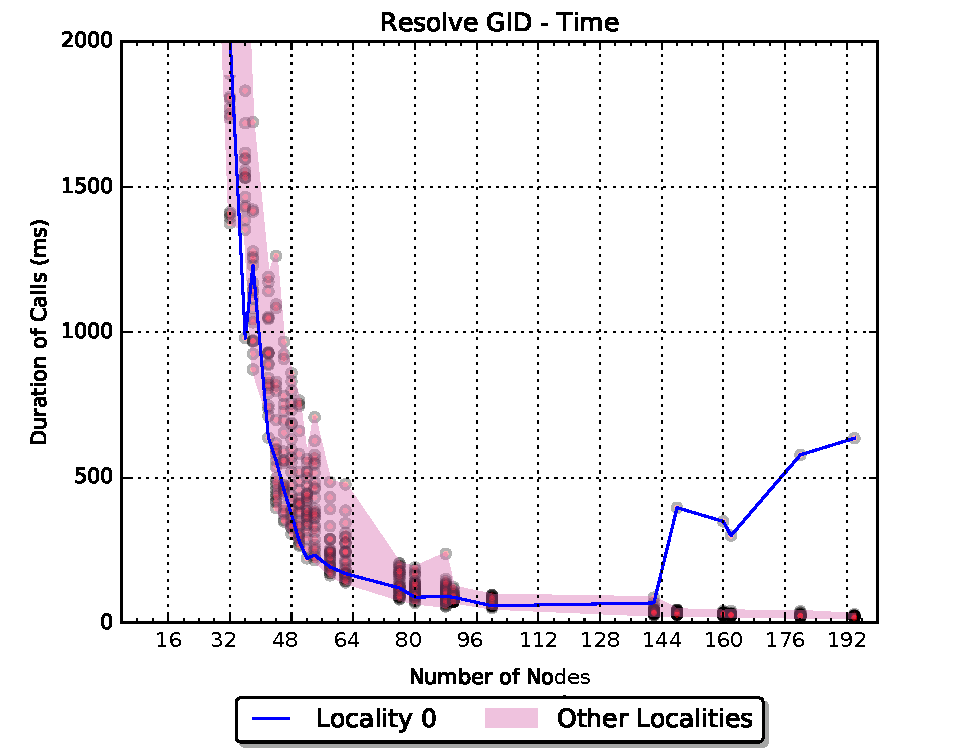
\includegraphics[width=.54\textwidth,height=\textheight,keepaspectratio]{graphs/octotiger_resolve_gid_time}
    \label{fig:octgr_strong_resolve_gid_time}
\end{figure}

Appropriate distribution of work is of particular interest to computer
scientists. In case of AGAS, ideally we expect the number of specific
operations and the amount of time spent to perform them to be similar. Address
resolution is one of the main functions of AGAS that translates a HPX GID to
the actual virtual address on a machine. Its operation is complicated if the
object is not currently located on the locality that address resolution is taking
place and in such case AGAS tries to determine which locality the object
currently lives on, serialize the task that asked to access the foreign GID in
an HPX parcel, and send it to the locality the object is living in. If an AGAS
instance has no knowledge of the locality that is holding an object then it
takes advantage of the fact that a locality on which an object is created stays
responsible for it during the object's entire lifetime and uses the metadata in
the GID to determine the locality on which the object was originally created and
sends the query there. Fig. \ref{fig:octgr_strong_resolve_gid_time} shows the
amount of time GID resolution takes while running OctoTiger. By looking at
the graph we notice that while the amount of work performed by each
locality is relatively similar up to 146 nodes, locality 0 starts to perform
more work than other localities. This may indicate that most objects globally
referenced were created on locality 0 and it requires further investigation to
determine if this effect is caused by application behavior, non-optimal data
distribution, or HPX itself.
% What else do I say?!

Parcels are the basic communication block in HPX. Parcels are active messages
that trigger an operation on the target AGAS instance that opens them and
usually contains a serialized task and its arguments. Parcel routing is the
operation in which the a parcel is sent to a different locality. Fig.
\ref{fig:octgr_strong_route_time} shows that locality 0 ends up handling a
disproportionate and increasing number of routing requests regardless of the
application data access pattern and problem size and hence, the routing operation
is a candidate for optimization.

\begin{figure}[h]
    \centering
    \caption{Total time spent to route calls while running OctoTiger on 2 to 200 nodes of SuperMIC with fixed problem size (Strong Scaling). Each (red) circle refers to the measured amount of time a locality has spent executing parcel route calls. Higher intensities indicate overlapping measurements. The line highlights locality 0's behavior.}
    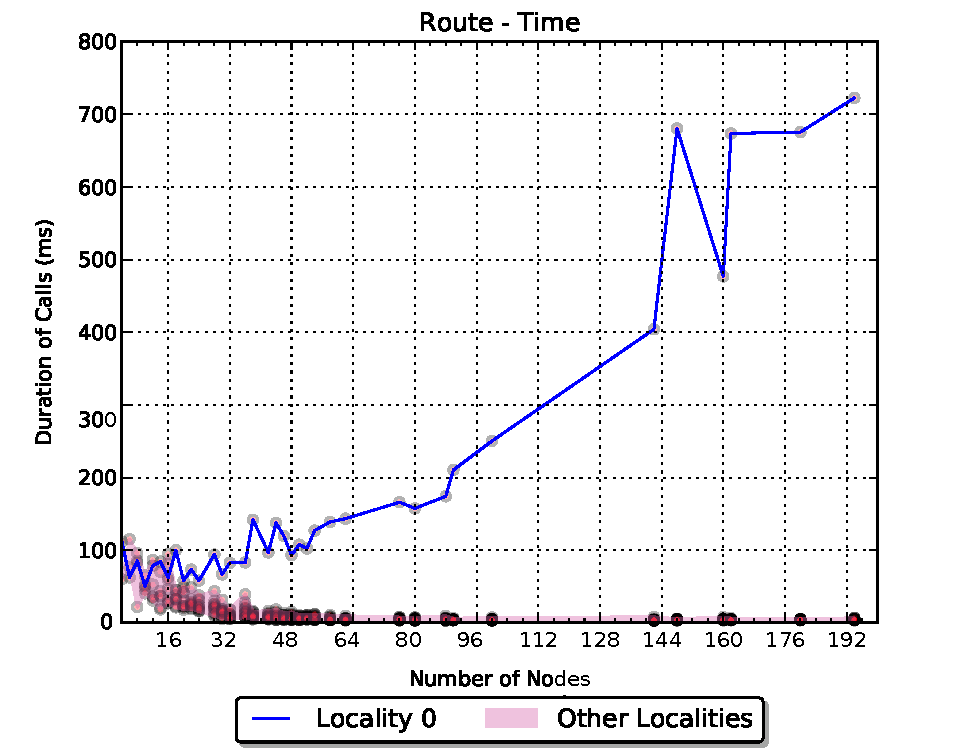
\includegraphics[width=.54\textwidth,height=\textheight,keepaspectratio]{graphs/octotiger_route_time}
    \label{fig:octgr_strong_route_time}
\end{figure}
% Garbage collection not done much in OctoTiger
For a garbage collection system to function the HPX runtime system must be able
to determine if an object is currently being used. HPX uses reference counting
for local references and a credit-based system to keep track of global
references. The operations that lend and return credits are called decrement
credit and increment credit, respectively.
%One issue that affects our
%experiment is that OctoTiger uses unmanaged objects and therefore AGAS garbage
%collection is not heavily relied upon and therefore the amount of time spent on
%global reference management is not a fair example of applications that do use
%garbage collection.  Despite this limitation, the large number of nodes and the
%limited usage of the operation still enables us to observe the changes in
%decrement credit's behavior as the number of nodes increase.
Fig \ref{fig:octgr_strong_decr_cred} depicts the behavior of decrement\_credit
calls that take place while running OctoTiger with the same number of objects as
the number of nodes are increased. This figure shows that a
linear increase in number of objects results in an exponential growth
in the amount of time spent on managing global references. Although this
behavior is likely to be different for applications that do not have as many
global references per each object and therefore decrement\_credit is a good
candidate for further optimizations.

\begin{figure}[h]
    \centering
    \caption{Total time spent to decrement calls while running OctoTiger on 2 to 200 nodes of SuperMIC with fixed problem size (Strong Scaling). Each (red) circle refers to the measured amount of time a locality has spent executing resolve GID calls. Higher intensities indicate overlapping measurements. The line highlights locality 0's behavior.}
    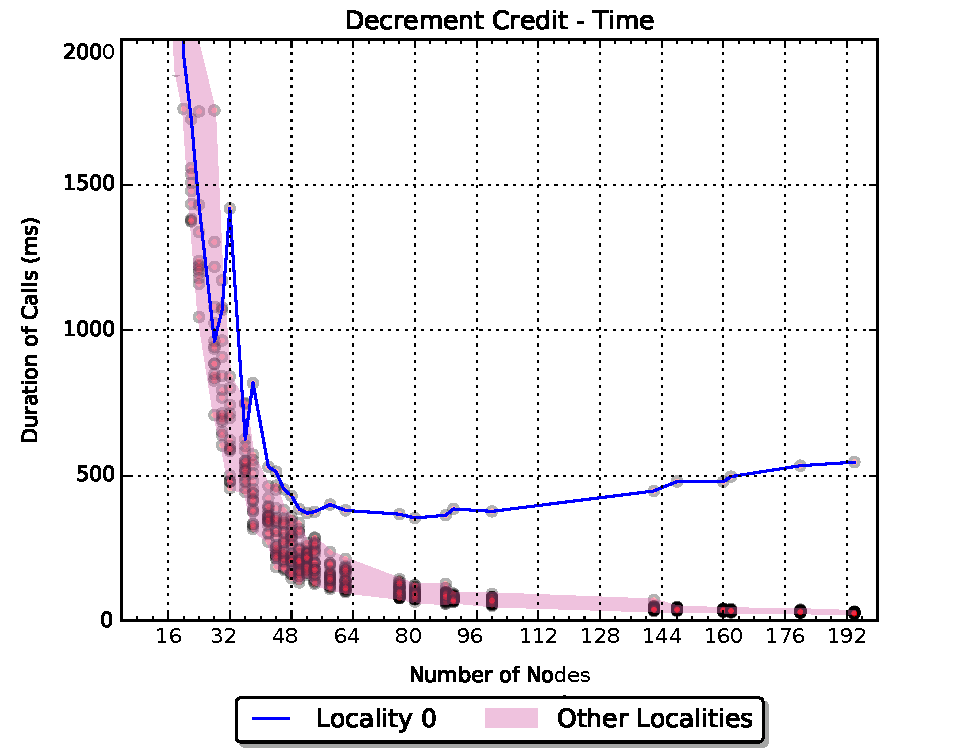
\includegraphics[width=.54\textwidth,height=\textheight,keepaspectratio]{graphs/octotiger_decrement_credit_time}
    \label{fig:octgr_strong_decr_cred}
\end{figure}

%\begin{figure}
%    \begin{subfigure}[b]{0.3\textwidth}
%        \centering
%        \caption{Total time spent to resolve GID calls while running OctoTiger on 2 to 200 nodes of SuperMIC with fixed problem size (Strong Scaling)}
%        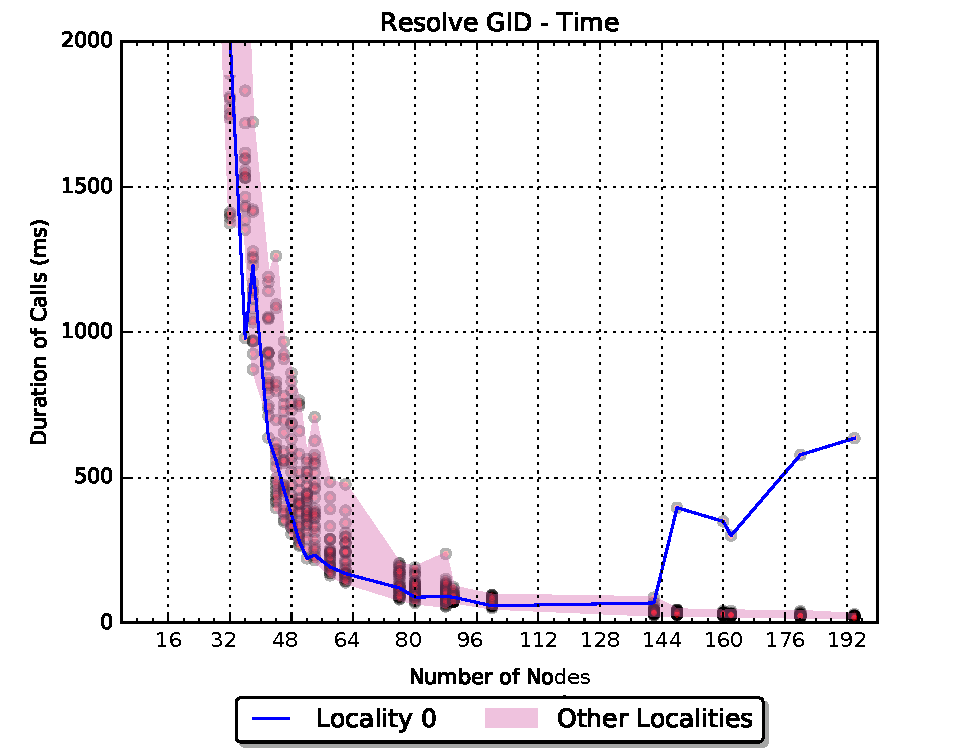
\includegraphics[width=\textwidth,keepaspectratio]{graphs/octotiger_resolve_gid_time}
%        \label{fig:octgr_strong_resolve_gid_time}
%    \end{subfigure}%
%    \hfill
%    \begin{subfigure}[b]{0.3\textwidth}
%        \caption{Total time spent to route calls while running OctoTiger on 2 to 200 nodes of SuperMIC with fixed problem size (Strong Scaling)}
%        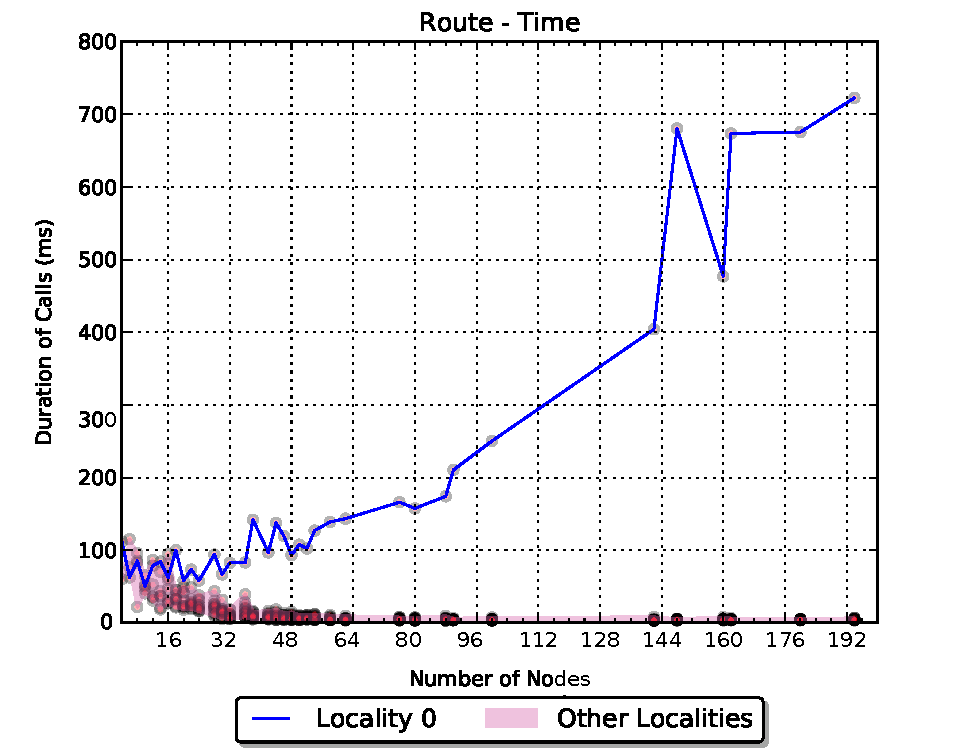
\includegraphics[width=\textwidth,height=\textheight,keepaspectratio]{graphs/octotiger_route_time}
%        \label{fig:octgr_strong_route_time}
%    \end{subfigure}%
%    \hfill
%    \begin{subfigure}[b]{0.3\textwidth}
%        \caption{Total time spent to decrement calls while running OctoTiger on 2 to 200 nodes of SuperMIC with fixed problem size (Strong Scaling)}
%        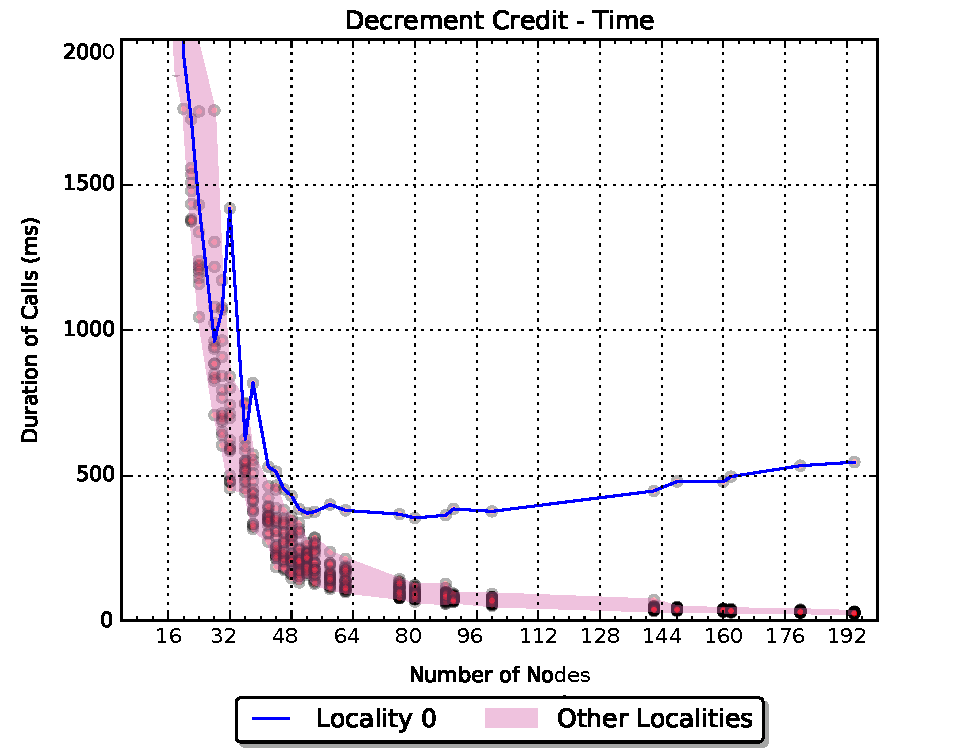
\includegraphics[width=\textwidth,height=\textheight,keepaspectratio]{graphs/octotiger_decrement_credit_time}
%        \label{fig:octgr_strong_decr_cred}
%    \end{subfigure}%
%\end{figure}


\section{Conclusions and Implications for Future Work}
\label{conclusions}

%\todo[inline, color=red!50]{
%Sketch: \\
%  Recap what was done. \\
%  Highlight accomplishments. \\
%  Conclude in way that feels like the work's finished. (Effects out of this work, any big questions) \\
%  Where do the results lead? \\
%  Keep it short \\
%  "just provide enough information as to a possible research path and why the path may be important" \\
%
%Should I mention there's an idea to put AGAS on hardware in the future?
%}

In this work we introduce AGAS, its subsystems, and a method to study how the
amount of time that is spent executing AGAS code, an overhead that does not
exist in PGAS systems that statically resolve global references during
compilation, is affected as the number of nodes increase.

To study AGAS's behavior we chose a multiphysics AMR application called
OctoTiger that generates and works with a significant number of objects. We
identify the performance metrics that reveal AGAS's performance and used the
corresponding counters in HPX's Performance Counter framework to collect
performance data from our strong scaling experiments.

Our observations show that in the cases of three basic AGAS operations, resolve
GID, route, and decrement credit, the AGAS instance on locality 0 performs an
increasing amount work as the problem is strongly scaled. Fig.
\ref{fig:octgr_strong_route_time} shows parcel routing as the operation that is
affected the most with an aggregated sum of $722$ milliseconds (0.0016\% of
execution time) spent on routing parcels by AGAS-invoked tasks on locality 0 on
200 nodes. Using our methods we were able to identify these issues which pose possible
performance bottlenecks that are being investigated and preliminary results
appear to show that this scaling issue has been addressed. Inclusion of a copy
of the locality namespace to each locality's AGAS cache in the current version
of HPX is one such optimization that reduces traffic forwarding to locality 0
due to not knowing the endpoint address for a locality.



% Original Template {{{ %
%\section{Fixed-Period Problems: The Sublinear Case}
%%
%With this chapter, the preliminaries are over, and we begin the search
%for periodic solutions to Hamiltonian systems. All this will be done in
%the convex case; that is, we shall study the boundary-value problem
%\begin{eqnarray*}
%  \dot{x}&=&JH' (t,x)\\
%  x(0) &=& x(T)
%\end{eqnarray*}
%with $H(t,\cdot)$ a convex function of $x$, going to $+\infty$ when
%$\left\|x\right\| \to \infty$.
%
%%
%\subsection{Autonomous Systems}
%%
%In this section, we will consider the case when the Hamiltonian $H(x)$
%is autonomous. For the sake of simplicity, we shall also assume that it
%is $C^{1}$.
%
%We shall first consider the question of nontriviality, within the
%general framework of
%$\left(A_{\infty},B_{\infty}\right)$-subquadratic Hamiltonians. In
%the second subsection, we shall look into the special case when $H$ is
%$\left(0,b_{\infty}\right)$-subquadratic,
%and we shall try to derive additional information.
%%
%\subsubsection{The General Case: Nontriviality.}
%%
%We assume that $H$ is
%$\left(A_{\infty},B_{\infty}\right)$-sub\-qua\-dra\-tic at infinity,
%for some constant symmetric matrices $A_{\infty}$ and $B_{\infty}$,
%with $B_{\infty}-A_{\infty}$ positive definite. Set:
%\begin{eqnarray}
%\gamma :&=&{\rm smallest\ eigenvalue\ of}\ \ B_{\infty} - A_{\infty} \\
%  \lambda : &=& {\rm largest\ negative\ eigenvalue\ of}\ \
%  J \frac{d}{dt} +A_{\infty}\ .
%\end{eqnarray}
%
%Theorem~\ref{ghou:pre} tells us that if $\lambda +\gamma < 0$, the
%boundary-value problem:
%\begin{equation}
%\begin{array}{rcl}
%  \dot{x}&=&JH' (x)\\
%  x(0)&=&x (T)
%\end{array}
%\end{equation}
%has at least one solution
%$\overline{x}$, which is found by minimizing the dual
%action functional:
%\begin{equation}
%  \psi (u) = \int_{o}^{T} \left[\frac{1}{2}
%  \left(\Lambda_{o}^{-1} u,u\right) + N^{\ast} (-u)\right] dt
%\end{equation}
%on the range of $\Lambda$, which is a subspace $R (\Lambda)_{L}^{2}$
%with finite codimension. Here
%\begin{equation}
%  N(x) := H(x) - \frac{1}{2} \left(A_{\infty} x,x\right)
%\end{equation}
%is a convex function, and
%\begin{equation}
%  N(x) \le \frac{1}{2}
%  \left(\left(B_{\infty} - A_{\infty}\right) x,x\right)
%  + c\ \ \ \forall x\ .
%\end{equation}
%
%%
%\begin{proposition}
%Assume $H'(0)=0$ and $ H(0)=0$. Set:
%\begin{equation}
%  \delta := \liminf_{x\to 0} 2 N (x) \left\|x\right\|^{-2}\ .
%  \label{eq:one}
%\end{equation}
%
%If $\gamma < - \lambda < \delta$,
%the solution $\overline{u}$ is non-zero:
%\begin{equation}
%  \overline{x} (t) \ne 0\ \ \ \forall t\ .
%\end{equation}
%\end{proposition}
%%
%\begin{proof}
%Condition (\ref{eq:one}) means that, for every
%$\delta ' > \delta$, there is some $\varepsilon > 0$ such that
%\begin{equation}
%  \left\|x\right\| \le \varepsilon \Rightarrow N (x) \le
%  \frac{\delta '}{2} \left\|x\right\|^{2}\ .
%\end{equation}
%
%It is an exercise in convex analysis, into which we shall not go, to
%show that this implies that there is an $\eta > 0$ such that
%\begin{equation}
%  f\left\|x\right\| \le \eta
%  \Rightarrow N^{\ast} (y) \le \frac{1}{2\delta '}
%  \left\|y\right\|^{2}\ .
%  \label{eq:two}
%\end{equation}
%
%\begin{figure}
%\vspace{2.5cm}
%\caption{This is the caption of the figure displaying a white eagle and
%a white horse on a snow field}
%\end{figure}
%
%Since $u_{1}$ is a smooth function, we will have
%$\left\|hu_{1}\right\|_\infty \le \eta$
%for $h$ small enough, and inequality (\ref{eq:two}) will hold,
%yielding thereby:
%\begin{equation}
%  \psi (hu_{1}) \le \frac{h^{2}}{2}
%  \frac{1}{\lambda} \left\|u_{1} \right\|_{2}^{2} + \frac{h^{2}}{2}
%  \frac{1}{\delta '} \left\|u_{1}\right\|^{2}\ .
%\end{equation}
%
%If we choose $\delta '$ close enough to $\delta$, the quantity
%$\left(\frac{1}{\lambda} + \frac{1}{\delta '}\right)$
%will be negative, and we end up with
%\begin{equation}
%  \psi (hu_{1}) < 0\ \ \ \ \ {\rm for}\ \ h\ne 0\ \ {\rm small}\ .
%\end{equation}
%
%On the other hand, we check directly that $\psi (0) = 0$. This shows
%that 0 cannot be a minimizer of $\psi$, not even a local one.
%So $\overline{u} \ne 0$ and
%$\overline{u} \ne \Lambda_{o}^{-1} (0) = 0$. \qed
%\end{proof}
%%
%\begin{corollary}
%Assume $H$ is $C^{2}$ and
%$\left(a_{\infty},b_{\infty}\right)$-subquadratic at infinity. Let
%$\xi_{1},\allowbreak\dots,\allowbreak\xi_{N}$  be the
%equilibria, that is, the solutions of $H' (\xi ) = 0$.
%Denote by $\omega_{k}$
%the smallest eigenvalue of $H'' \left(\xi_{k}\right)$, and set:
%\begin{equation}
%  \omega : = {\rm Min\,} \left\{\omega_{1},\dots,\omega_{k}\right\}\ .
%\end{equation}
%If:
%\begin{equation}
%  \frac{T}{2\pi} b_{\infty} <
%  - E \left[- \frac{T}{2\pi}a_{\infty}\right] <
%  \frac{T}{2\pi}\omega
%  \label{eq:three}
%\end{equation}
%then minimization of $\psi$ yields a non-constant $T$-periodic solution
%$\overline{x}$.
%\end{corollary}
%%
%
%We recall once more that by the integer part $E [\alpha ]$ of
%$\alpha \in \bbbr$, we mean the $a\in \bbbz$
%such that $a< \alpha \le a+1$. For instance,
%if we take $a_{\infty} = 0$, Corollary 2 tells
%us that $\overline{x}$ exists and is
%non-constant provided that:
%
%\begin{equation}
%  \frac{T}{2\pi} b_{\infty} < 1 < \frac{T}{2\pi}
%\end{equation}
%or
%\begin{equation}
%  T\in \left(\frac{2\pi}{\omega},\frac{2\pi}{b_{\infty}}\right)\ .
%  \label{eq:four}
%\end{equation}
%
%%
%\begin{proof}
%The spectrum of $\Lambda$ is $\frac{2\pi}{T} \bbbz +a_{\infty}$. The
%largest negative eigenvalue $\lambda$ is given by
%$\frac{2\pi}{T}k_{o} +a_{\infty}$,
%where
%\begin{equation}
%  \frac{2\pi}{T}k_{o} + a_{\infty} < 0
%  \le \frac{2\pi}{T} (k_{o} +1) + a_{\infty}\ .
%\end{equation}
%Hence:
%\begin{equation}
%  k_{o} = E \left[- \frac{T}{2\pi} a_{\infty}\right] \ .
%\end{equation}
%
%The condition $\gamma < -\lambda < \delta$ now becomes:
%\begin{equation}
%  b_{\infty} - a_{\infty} <
%  - \frac{2\pi}{T} k_{o} -a_{\infty} < \omega -a_{\infty}
%\end{equation}
%which is precisely condition (\ref{eq:three}).\qed
%\end{proof}
%%
%
%\begin{lemma}
%Assume that $H$ is $C^{2}$ on $\bbbr^{2n} \setminus \{ 0\}$ and
%that $H'' (x)$ is non-de\-gen\-er\-ate for any $x\ne 0$. Then any local
%minimizer $\widetilde{x}$ of $\psi$ has minimal period $T$.
%\end{lemma}
%%
%\begin{proof}
%We know that $\widetilde{x}$, or
%$\widetilde{x} + \xi$ for some constant $\xi
%\in \bbbr^{2n}$, is a $T$-periodic solution of the Hamiltonian system:
%\begin{equation}
%  \dot{x} = JH' (x)\ .
%\end{equation}
%
%There is no loss of generality in taking $\xi = 0$. So
%$\psi (x) \ge \psi (\widetilde{x} )$
%for all $\widetilde{x}$ in some neighbourhood of $x$ in
%$W^{1,2} \left(\bbbr / T\bbbz ; \bbbr^{2n}\right)$.
%
%But this index is precisely the index
%$i_{T} (\widetilde{x} )$ of the $T$-periodic
%solution $\widetilde{x}$ over the interval
%$(0,T)$, as defined in Sect.~2.6. So
%\begin{equation}
%  i_{T} (\widetilde{x} ) = 0\ .
%  \label{eq:five}
%\end{equation}
%
%Now if $\widetilde{x}$ has a lower period, $T/k$ say,
%we would have, by Corollary 31:
%\begin{equation}
%  i_{T} (\widetilde{x} ) =
%  i_{kT/k}(\widetilde{x} ) \ge
%  ki_{T/k} (\widetilde{x} ) + k-1 \ge k-1 \ge 1\ .
%\end{equation}
%
%This would contradict (\ref{eq:five}), and thus cannot happen.\qed
%\end{proof}
%%
%\paragraph{Notes and Comments.}
%The results in this section are a
%refined version of \cite{clar:eke};
%the minimality result of Proposition
%14 was the first of its kind.
%
%To understand the nontriviality conditions, such as the one in formula
%(\ref{eq:four}), one may think of a one-parameter family
%$x_{T}$, $T\in \left(2\pi\omega^{-1}, 2\pi b_{\infty}^{-1}\right)$
%of periodic solutions, $x_{T} (0) = x_{T} (T)$,
%with $x_{T}$ going away to infinity when $T\to 2\pi \omega^{-1}$,
%which is the period of the linearized system at 0.
%
%\begin{table}
%\caption{This is the example table taken out of {\it The
%\TeX{}book,} p.\,246}
%\begin{center}
%\begin{tabular}{r@{\quad}rl}
%\hline
%\multicolumn{1}{l}{\rule{0pt}{12pt}
%                   Year}&\multicolumn{2}{l}{World population}\\[2pt]
%\hline\rule{0pt}{12pt}
%8000 B.C.  &     5,000,000& \\
%  50 A.D.  &   200,000,000& \\
%1650 A.D.  &   500,000,000& \\
%1945 A.D.  & 2,300,000,000& \\
%1980 A.D.  & 4,400,000,000& \\[2pt]
%\hline
%\end{tabular}
%\end{center}
%\end{table}
%%
%\begin{theorem} [Ghoussoub-Preiss]\label{ghou:pre}
%Assume $H(t,x)$ is
%$(0,\varepsilon )$-subquadratic at
%infinity for all $\varepsilon > 0$, and $T$-periodic in $t$
%\begin{equation}
%  H (t,\cdot )\ \ \ \ \ {\rm is\ convex}\ \ \forall t
%\end{equation}
%\begin{equation}
%  H (\cdot ,x)\ \ \ \ \ {\rm is}\ \ T{\rm -periodic}\ \ \forall x
%\end{equation}
%\begin{equation}
%  H (t,x)\ge n\left(\left\|x\right\|\right)\ \ \ \ \
%  {\rm with}\ \ n (s)s^{-1}\to \infty\ \ {\rm as}\ \ s\to \infty
%\end{equation}
%\begin{equation}
%  \forall \varepsilon > 0\ ,\ \ \ \exists c\ :\
%  H(t,x) \le \frac{\varepsilon}{2}\left\|x\right\|^{2} + c\ .
%\end{equation}
%
%Assume also that $H$ is $C^{2}$, and $H'' (t,x)$ is positive definite
%everywhere. Then there is a sequence $x_{k}$, $k\in \bbbn$, of
%$kT$-periodic solutions of the system
%\begin{equation}
%  \dot{x} = JH' (t,x)
%\end{equation}
%such that, for every $k\in \bbbn$, there is some $p_{o}\in\bbbn$ with:
%\begin{equation}
%  p\ge p_{o}\Rightarrow x_{pk} \ne x_{k}\ .
%\end{equation}
%\qed
%\end{theorem}
%%
%\begin{example} [{{\rm External forcing}}]
%Consider the system:
%\begin{equation}
%  \dot{x} = JH' (x) + f(t)
%\end{equation}
%where the Hamiltonian $H$ is
%$\left(0,b_{\infty}\right)$-subquadratic, and the
%forcing term is a distribution on the circle:
%\begin{equation}
%  f = \frac{d}{dt} F + f_{o}\ \ \ \ \
%  {\rm with}\ \ F\in L^{2} \left(\bbbr / T\bbbz; \bbbr^{2n}\right)\ ,
%\end{equation}
%where $f_{o} : = T^{-1}\int_{o}^{T} f (t) dt$. For instance,
%\begin{equation}
%  f (t) = \sum_{k\in \bbbn} \delta_{k} \xi\ ,
%\end{equation}
%where $\delta_{k}$ is the Dirac mass at $t= k$ and
%$\xi \in \bbbr^{2n}$ is a
%constant, fits the prescription. This means that the system
%$\dot{x} = JH' (x)$ is being excited by a
%series of identical shocks at interval $T$.
%\end{example}
%%
%\begin{definition}
%Let $A_{\infty} (t)$ and $B_{\infty} (t)$ be symmetric
%operators in $\bbbr^{2n}$, depending continuously on
%$t\in [0,T]$, such that
%$A_{\infty} (t) \le B_{\infty} (t)$ for all $t$.
%
%A Borelian function
%$H: [0,T]\times \bbbr^{2n} \to \bbbr$
%is called
%$\left(A_{\infty} ,B_{\infty}\right)$-{\it subquadratic at infinity}
%if there exists a function $N(t,x)$ such that:
%\begin{equation}
%  H (t,x) = \frac{1}{2} \left(A_{\infty} (t) x,x\right) + N(t,x)
%\end{equation}
%\begin{equation}
%  \forall t\ ,\ \ \ N(t,x)\ \ \ \ \
%  {\rm is\ convex\ with\  respect\  to}\ \ x
%\end{equation}
%\begin{equation}
%  N(t,x) \ge n\left(\left\|x\right\|\right)\ \ \ \ \
%  {\rm with}\ \ n(s)s^{-1}\to +\infty\ \ {\rm as}\ \ s\to +\infty
%\end{equation}
%\begin{equation}
%  \exists c\in \bbbr\ :\ \ \ H (t,x) \le
%  \frac{1}{2} \left(B_{\infty} (t) x,x\right) + c\ \ \ \forall x\ .
%\end{equation}
%
%If $A_{\infty} (t) = a_{\infty} I$ and
%$B_{\infty} (t) = b_{\infty} I$, with
%$a_{\infty} \le b_{\infty} \in \bbbr$,
%we shall say that $H$ is
%$\left(a_{\infty},b_{\infty}\right)$-subquadratic
%at infinity. As an example, the function
%$\left\|x\right\|^{\alpha}$, with
%$1\le \alpha < 2$, is $(0,\varepsilon )$-subquadratic at infinity
%for every $\varepsilon > 0$. Similarly, the Hamiltonian
%\begin{equation}
%H (t,x) = \frac{1}{2} k \left\|k\right\|^{2} +\left\|x\right\|^{\alpha}
%\end{equation}
%is $(k,k+\varepsilon )$-subquadratic for every $\varepsilon > 0$.
%Note that, if $k<0$, it is not convex.
%\end{definition}
%%
%
%\paragraph{Notes and Comments.}
%The first results on subharmonics were
%obtained by Rabinowitz in \cite{rab}, who showed the existence of
%infinitely many subharmonics both in the subquadratic and superquadratic
%case, with suitable growth conditions on $H'$. Again the duality
%approach enabled Clarke and Ekeland in \cite{clar:eke:2} to treat the
%same problem in the convex-subquadratic case, with growth conditions on
%$H$ only.
%
%Recently, Michalek and Tarantello (see \cite{mich:tar} and \cite{tar})
%have obtained lower bound on the number of subharmonics of period $kT$,
%based on symmetry considerations and on pinching estimates, as in
%Sect.~5.2 of this article.
% }}} Original Template %

%
% ---- Bibliography ----
%
\bibliographystyle{splncs03}
\bibliography{references} 
%\begin{thebibliography}{5}
%%
%\bibitem {clar:eke}
%Clarke, F., Ekeland, I.:
%Nonlinear oscillations and
%boundary-value problems for Hamiltonian systems.
%Arch. Rat. Mech. Anal. 78, 315--333 (1982)
%
%\bibitem {clar:eke:2}
%Clarke, F., Ekeland, I.:
%Solutions p\'{e}riodiques, du
%p\'{e}riode donn\'{e}e, des \'{e}quations hamiltoniennes.
%Note CRAS Paris 287, 1013--1015 (1978)
%
%\bibitem {mich:tar}
%Michalek, R., Tarantello, G.:
%Subharmonic solutions with prescribed minimal
%period for nonautonomous Hamiltonian systems.
%J. Diff. Eq. 72, 28--55 (1988)
%
%\bibitem {tar}
%Tarantello, G.:
%Subharmonic solutions for Hamiltonian
%systems via a $\bbbz_{p}$ pseudoindex theory.
%Annali di Matematica Pura (to appear)
%
%\bibitem {rab}
%Rabinowitz, P.:
%On subharmonic solutions of a Hamiltonian system.
%Comm. Pure Appl. Math. 33, 609--633 (1980)
%
%\end{thebibliography}
\end{document}
